\clearpage
\begin{figure}[H]\centering
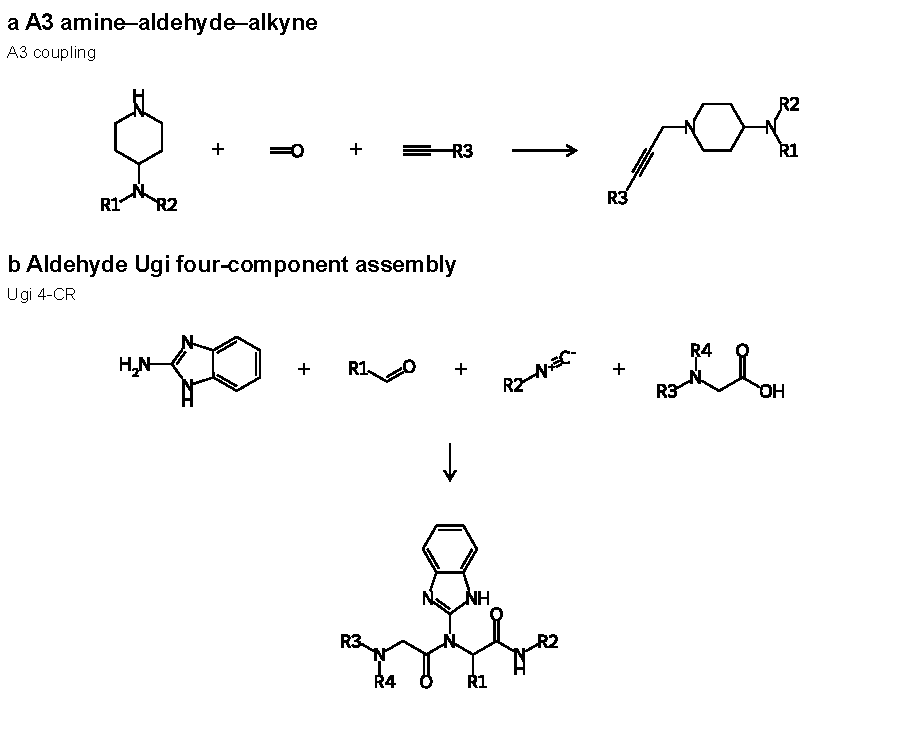
\includegraphics[width=\linewidth,height=.80\textheight,keepaspectratio]{figures/all_family_reactions/multicomponent_a.pdf}
\caption{\textbf{Multicomponent assembly: A3 and Ugi four-component reactions.}
\textbf{a}, A3 coupling creates C--N and C--C bonds while retaining the alkyne.
\textbf{b}, Aldehyde Ugi 4-CR combines an amine, aldehyde, isocyanide and carboxylic acid.
The acid supplies the N-acyl unit in the four-component reaction.}
\label{fig:rxn-multicomponent-a}\end{figure}

\clearpage
\begin{figure}[H]\centering
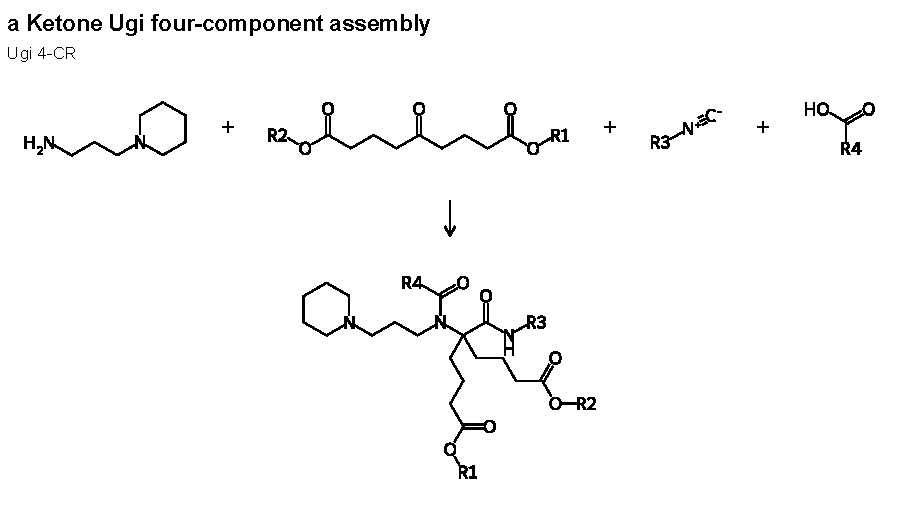
\includegraphics[width=\linewidth,height=.80\textheight,keepaspectratio]{figures/all_family_reactions/ketone_ugi4.pdf}
\caption{\textbf{Ketone Ugi four-component assembly.} The ketone reacts with an amine, isocyanide
and carboxylic acid. Both carbon substituents remain attached to the ketone-derived center; the
preassembled ester-bearing arms are retained, and the acid supplies the N-acyl unit.}
\label{fig:rxn-ketone-ugi4}\end{figure}

\clearpage
\begin{figure}[H]\centering
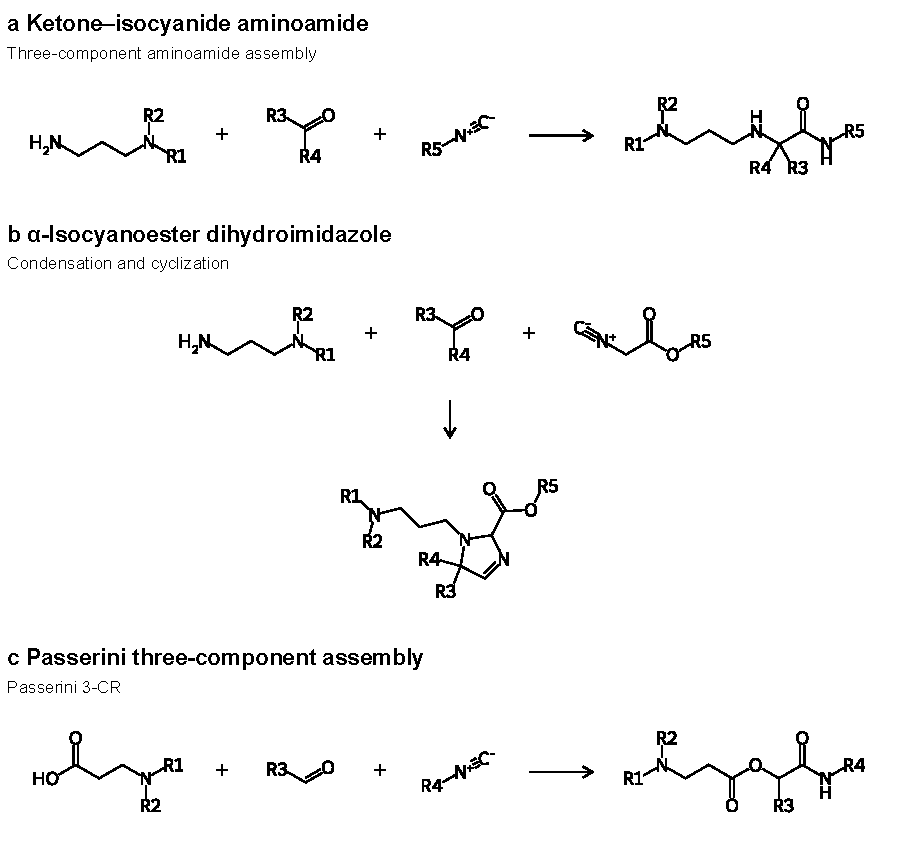
\includegraphics[width=\linewidth,height=.80\textheight,keepaspectratio]{figures/all_family_reactions/multicomponent_b.pdf}
\caption{\textbf{Multicomponent assembly: aminoamide, dihydroimidazole and Passerini reactions.}
\textbf{a}, The ketone--isocyanide branch forms an aminoamide from three components.
\textbf{b}, An $\alpha$-isocyanoester participates in dihydroimidazole ring formation, retaining its ester.
\textbf{c}, Passerini assembly produces an $\alpha$-acyloxy amide from an aldehyde, acid and isocyanide;
the acid-derived acyl group attaches through oxygen.}
\label{fig:rxn-multicomponent-b}\end{figure}

\clearpage
\begin{figure}[H]\centering
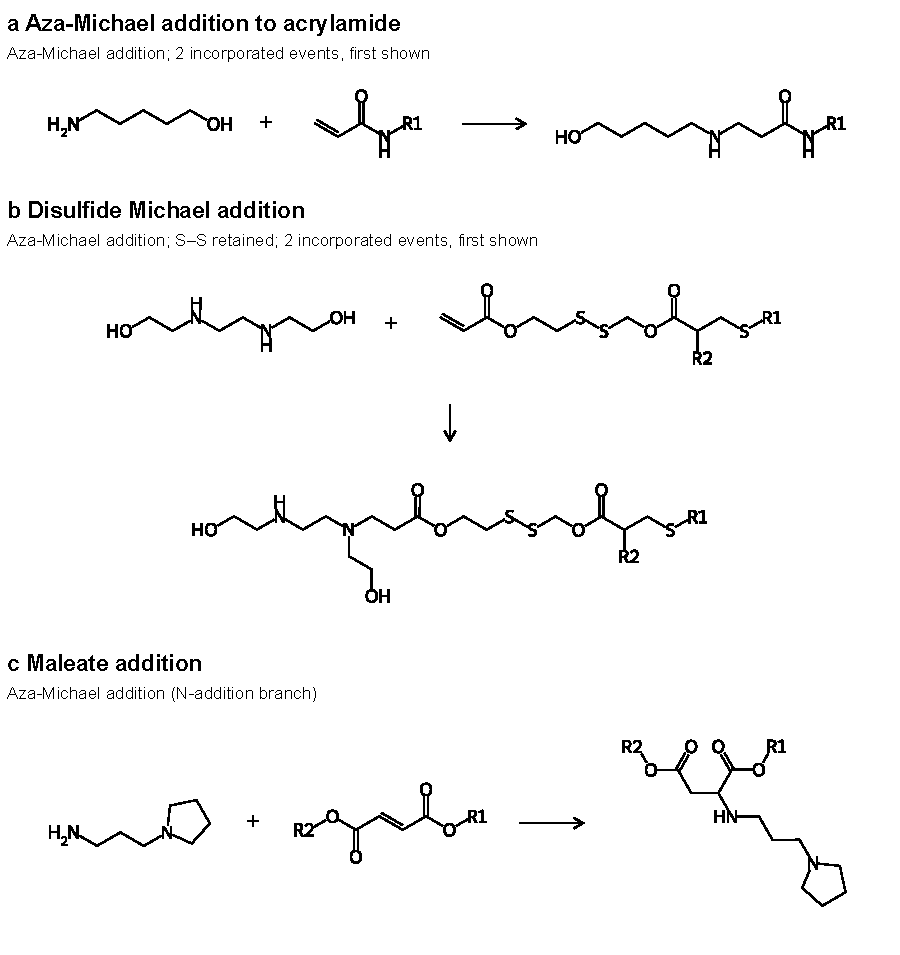
\includegraphics[width=\linewidth,height=.80\textheight,keepaspectratio]{figures/all_family_reactions/conjugate_additions.pdf}
\caption{\textbf{Conjugate-addition families.}
\textbf{a}, Amine addition to an acrylamide retains the amide interface.
\textbf{b}, Addition to a disulfide-containing acrylate retains its S--S bond.
\textbf{c}, The illustrated maleate program uses the N-addition branch and retains both ester groups.
For repeated programs, one event is shown and the incorporated-event count is indicated.
The aza-Michael acrylate reaction is shown in Figure~\ref{fig:reaction-schemes}.}
\label{fig:rxn-conjugate}\end{figure}

\clearpage
\begin{figure}[H]\centering
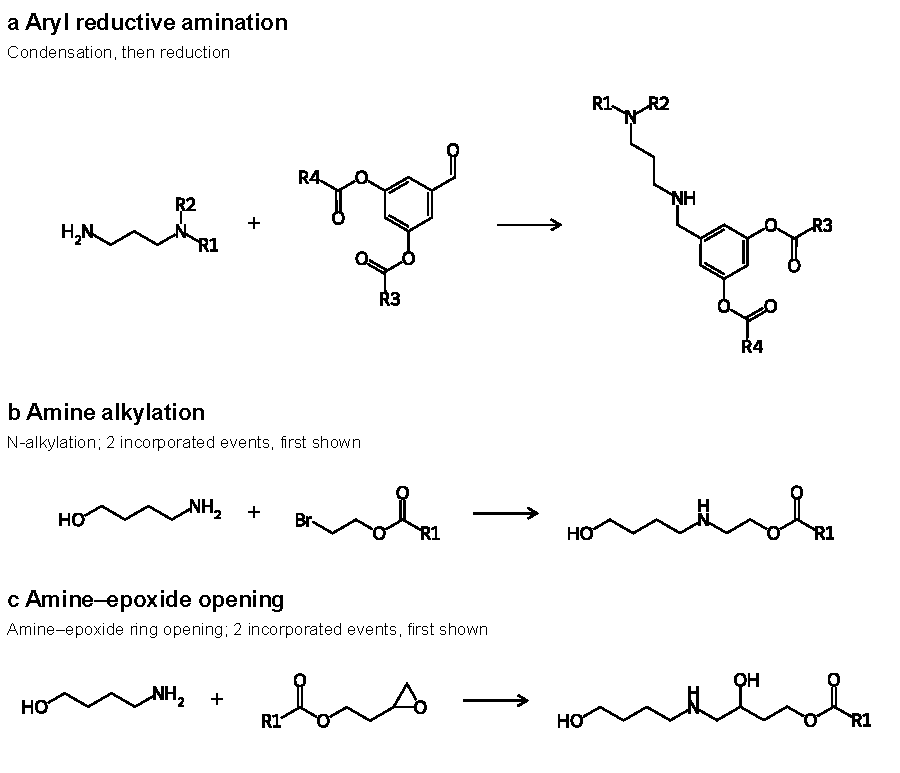
\includegraphics[width=\linewidth,height=.80\textheight,keepaspectratio]{figures/all_family_reactions/functionalization.pdf}
\caption{\textbf{Nitrogen functionalization.}
\textbf{a}, Aryl reductive amination combines condensation with reduction.
\textbf{b}, N-alkylation replaces the alkyl bromide leaving group.
\textbf{c}, Amine attack opens an epoxide and retains the resulting alcohol.
Repeated incorporations are labeled.}
\label{fig:rxn-functionalization}\end{figure}

\clearpage
\begin{figure}[H]\centering
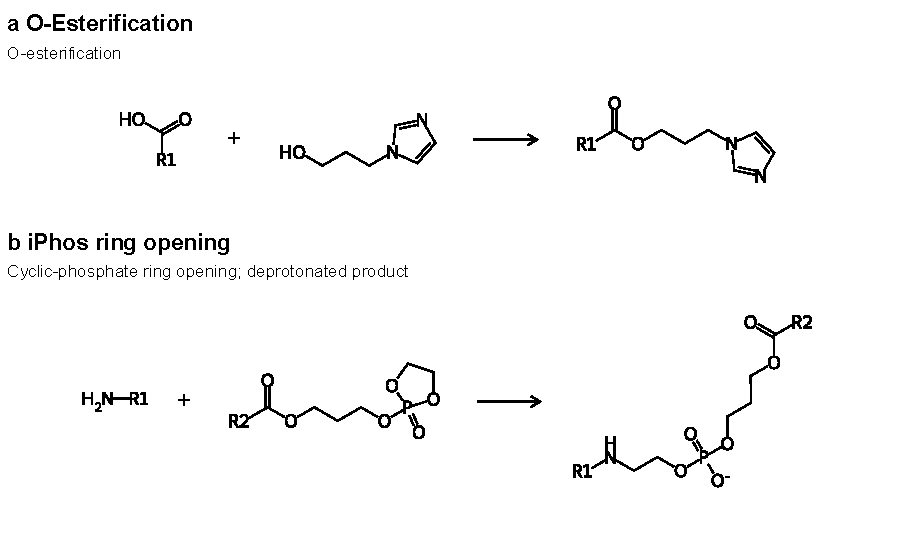
\includegraphics[width=\linewidth,height=.80\textheight,keepaspectratio]{figures/all_family_reactions/oxygen_phosphate.pdf}
\caption{\textbf{Esterification and phosphate opening.}
\textbf{a}, O-esterification joins an aminoalcohol to an acid while retaining the basic nitrogen.
\textbf{b}, iPhos assembly opens a C--O bond of a cyclic phosphate to form the N--CH$_2$CH$_2$--O--P
connection. Its deprotonated product representation is preserved.}
\label{fig:rxn-oxygen-phosphate}\end{figure}

\clearpage
\begin{figure}[H]\centering
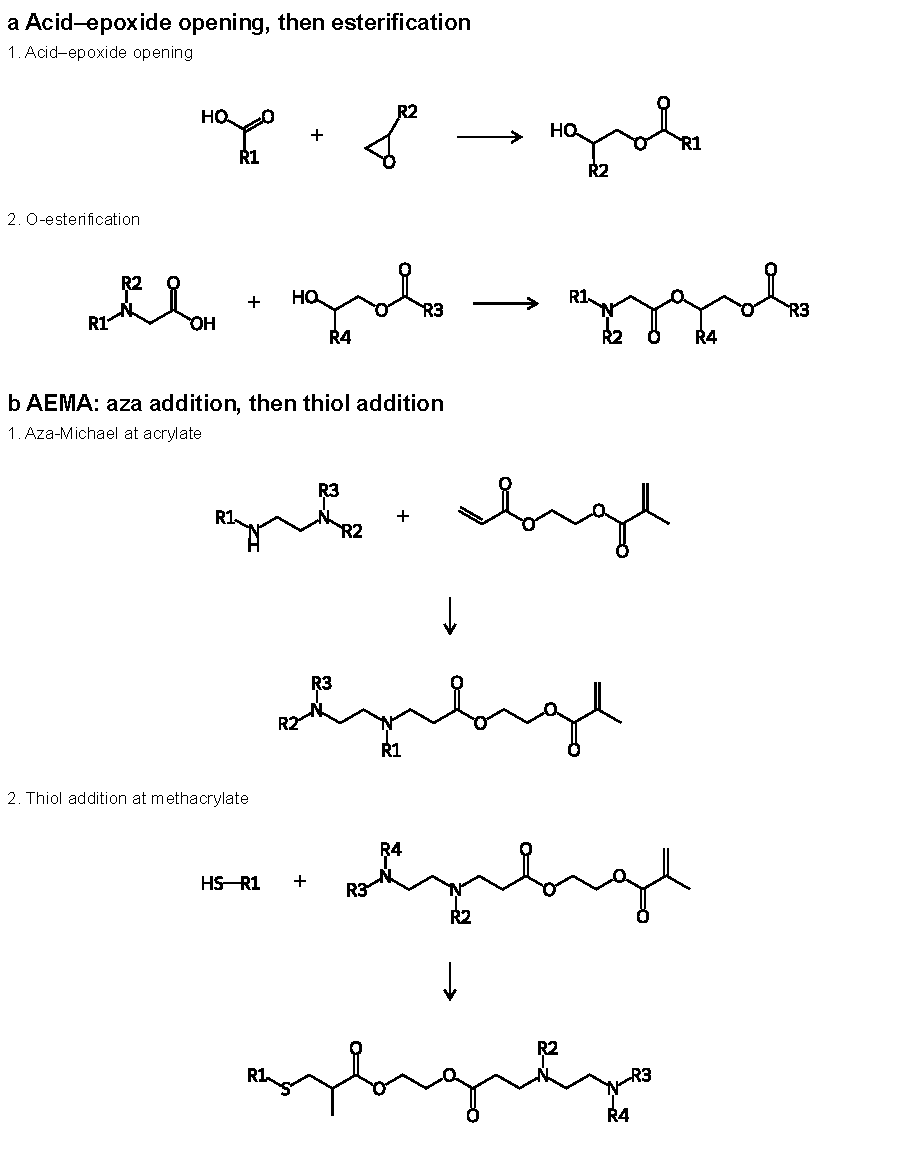
\includegraphics[width=\linewidth,height=.80\textheight,keepaspectratio]{figures/all_family_reactions/ordered_assemblies_a.pdf}
\caption{\textbf{Ordered assembly through hydroxy-ester and dual-acceptor intermediates.}
\textbf{a}, Acid--epoxide opening first produces a hydroxy ester; subsequent esterification attaches
the aminoacid head through its carboxyl group.
\textbf{b}, The AEMA program consumes the acrylate in an aza-Michael addition, then the remaining
methacrylate in a thiol addition. Each second-stage reactant is the corresponding first-stage
intermediate; $R$ abbreviations are local to each arrow.}
\label{fig:rxn-ordered-a}\end{figure}

\clearpage
\begin{figure}[H]\centering
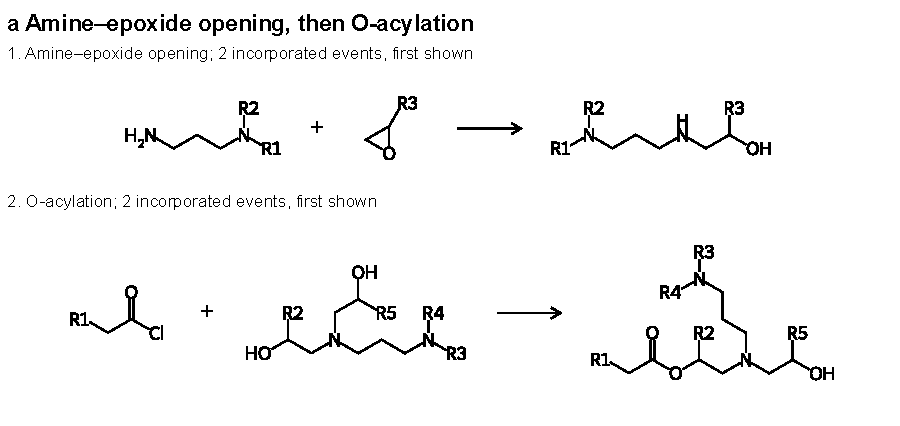
\includegraphics[width=\linewidth,height=.80\textheight,keepaspectratio]{figures/all_family_reactions/ordered_assemblies_b.pdf}
\caption{\textbf{Epoxide opening followed by O-acylation.}
Amine--epoxide additions first form aminoalcohol arms. The resulting alcohols then react with acyl
chlorides to form ester linkages. The representative program incorporates two epoxides and two
acyl groups; one event from each stage is drawn, with its multiplicity indicated.}
\label{fig:rxn-ordered-b}\end{figure}

\clearpage
\begin{figure}[H]\centering
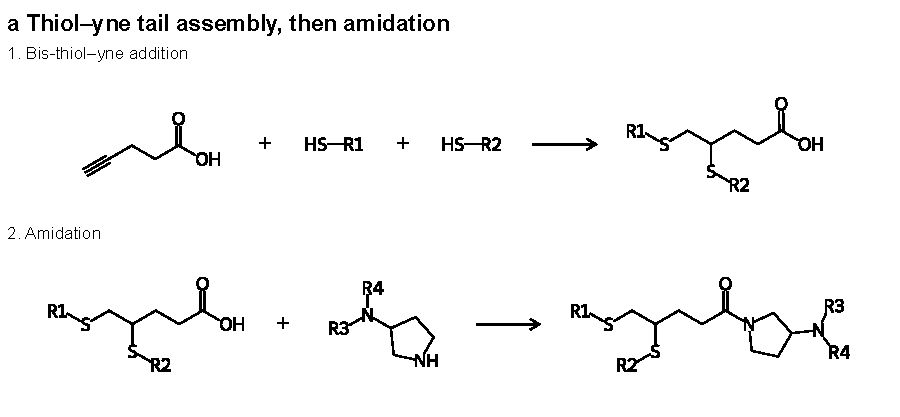
\includegraphics[width=\linewidth,height=.80\textheight,keepaspectratio]{figures/all_family_reactions/ordered_assemblies_c.pdf}
\caption{\textbf{Thiol--yne tail assembly followed by amidation.}
Two identical thiols ($R_1=R_2$ within each arrow) add across a terminal alkyne to form the
bis(thioether) acid, which then undergoes amidation. The first arrow denotes the net double addition.}
\label{fig:rxn-ordered-c}\end{figure}

\clearpage
\begin{figure}[H]\centering
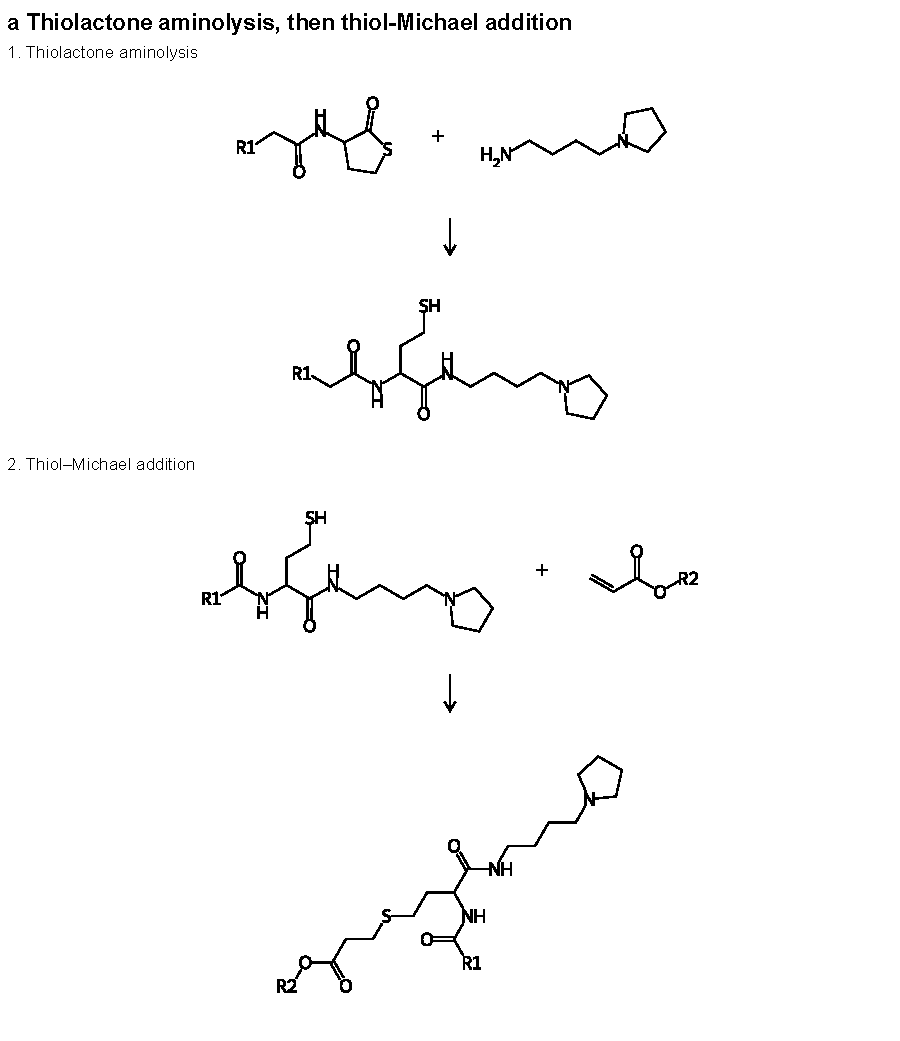
\includegraphics[width=\linewidth,height=.80\textheight,keepaspectratio]{figures/all_family_reactions/ordered_assemblies_d.pdf}
\caption{\textbf{Thiolactone aminolysis followed by thiol--Michael addition.}
Aminolysis opens the thiolactone to form an amide and release a thiol. The subsequent addition
to an acrylate forms a thioether. The retained sulfur framework distinguishes this transformation
from disulfide formation.}
\label{fig:rxn-ordered-d}\end{figure}
